\documentclass[12pt,a4paper]{article}
\usepackage{verbatim}
\usepackage{graphicx}
\usepackage{amsmath}
\usepackage{float}
\author{ZHANG Xiao Research Intern in IBM CRL}
\title{Network 20q HW5	}

\begin{document}
\maketitle
\pagebreak

\section{Contagion}
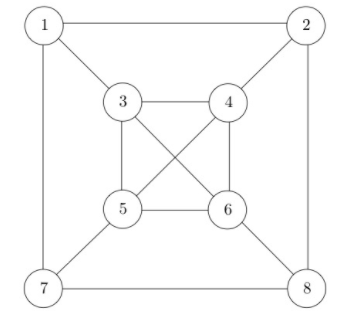
\includegraphics{PIC/1.png}
\subsection{a}
Under this situation, node 1 flip to 1, and other nodes stay in 0. The nodes adjacent to node 1 (that is 2, 3, 7) could change. $d_2 = \frac{1}{3} > 0.3$, $d_3 = \frac{1}{4} < 0.3$ and $d_7 = \frac{1}{3} > 0.3$. So in the first round, node 2 and node 7 change to state-1.

While in the second round, 3, 5, 4, 8 could change.  $d_3 = \frac{1}{4} < 0.3$,  $d_5 = \frac{1}{4} < 0.3$,  $d_4 = \frac{1}{4} < 0.3$,  $d_8 = \frac{2}{3} > 0.3$.
So in this round, node 8 would flip to state-1.

In the following round, node 1,2,7,8 stay in state 1, node 3,4,5,6 stay in state 0, because their density would stay in $\frac{1}{4}$ and would not be larger than $p$.
\subsection{b}
While start at node 3, in round 1, node 1 would flip to state 1. In the next round, node 2 and 7 would change to state 1. In the third round, node 4, 5, 8 change to state 1, in the last round, node 6 change to state 1.

\subsection{c}
In a, only the outer layer of the graph change to 1  in the end, but in b all nodes change to 1 in the end. We could split this graph's nodes into two clusters, cluster 1 includes node 1,2,7,8 and the density is 2/3. cluster 2 includes node 3,4,5,6 and the density is 3/4. So when $ p=0.3 $, the 1 node in outer layer could not make cluster 2 to change, because $D_{3,4,5,6} = \frac{3}{4} > 1-p = 0.7$. But when node 3 change to 1 the adjacent cluster 1 $D_{1,2,7,8} = \frac{2}{3} < 1-p = 0.7$, so cluster 1 would be infected in the end.
\section{De Bruijin Sequence}
In this question, we could build De Bruijin graph, while $k=1 and k=2$, the graph is like:

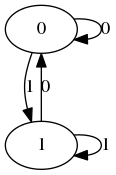
\includegraphics{PIC/DBg1.png}
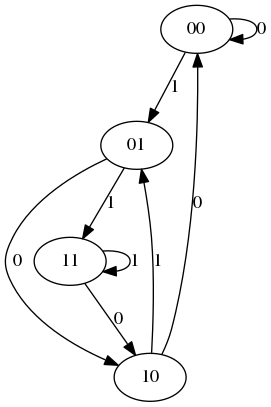
\includegraphics{PIC/DBg2.png}

The node is encoden with the length of k, and it could define the maximum nodes in the graph. And each node could accept a one-bit input, then drift to other node append with current bit to the end and drop the first bit in the head.

From above graphs, we could see that for each node in the graph the in-degree is equal to out-degree and is 2. Because for a k length bits, it could only accept 2 kinds of input, 0 and 1, and the out-degree could be the first bit dropped as 0 and 1. So the in-degree and out-degree for each node in De Bruijin graph is 2. So for any order k, there exist Bruijn sequence.

And to get a Bruijin sequence, just traverse the graph and cover all the edges only once would get the sequence. 

\end{document}